%
% Modelo de relatório/trabalho
%
\documentclass[a4paper, 12pt]{article}

\usepackage[portuguese]{babel}
\usepackage[utf8]{inputenc}
\usepackage[T1]{fontenc}
\usepackage{array}
\usepackage{fixltx2e}
\usepackage{amsmath}
\usepackage{amssymb}
\usepackage{graphicx}
\usepackage{caption}
\usepackage{subcaption}
\usepackage{float}
\usepackage{a4wide}
\usepackage{courier}
\usepackage{multicol}
\usepackage[table]{xcolor}
\usepackage[htt]{hyphenat}
\usepackage{makeidx}
\usepackage{hyperref}
\usepackage{setspace}
\usepackage{indentfirst}
\usepackage[nottoc]{tocbibind}
\usepackage{listings}
\usepackage[bottom]{footmisc}
\usepackage[a4paper,top=2.0cm,bottom=2.0cm,left=1.83cm,right=2.0cm]{geometry}
\usepackage[square, sort, comma, numbers]{natbib}

\onehalfspacing
\graphicspath{{../diagrams/}}
\makeindex

\lstset{
    basicstyle=\footnotesize,
    morekeywords={either,or,transform,rule,to,from,through,function},
    frame=L,
}

\setcounter{secnumdepth}{2}
\setcounter{tocdepth}{2}

\begin{document}

\hypersetup{backref,pdfpagemode=FullScreen,colorlinks=true}

\title{EP1 --- MAC5742}
\author{Thilo Koch e Pedro Bruel}
\date{}
\maketitle

\section{Introdução} \label{sec:intro}

Este relatório descreve as atividades realizadas
para o EP1 da disciplina de Computação Paralela e
Distribuída (\textit{MAC5742}). A Seção \ref{sec:ex1}
descreve e corrige um exemplo encontrado num tutorial do padrão
OpenMP, e a Seção \ref{sec:ex2} descreve as modificações,
experimentos e interpretações feitos no código fornecido no enunciado.

Os diretórios \texttt{src}, \texttt{failing-example} e \texttt{doc}
contêm \textit{Makefiles} para geração dos executáveis e da documentação,
portanto basta executar o comando \texttt{make} para gerá-los.

\section{Exercício 1} \label{sec:ex1}

Neste exercício, procuramos um exemplo que contivesse falhas em um
tutorial, e tentamos corrigi-lo. O código do exemplo está na Seção
\ref{sec:example}, e nossa correção na Seção \ref{sec:fixed}.

Seguindo manual \textit{Guide into OpenMP: Easy multithreading
programming for C++}, na seção sobre OpenMP e \textit{fork()}
\footnotemark[1],
encontramos um exemplo que usa uma chamada a \textit{fork()} para criar um
subprocesso que utiliza cláusulas OpenMP.

O exemplo tem a intenção de demonstrar o uso \textit{incorreto} do OpenMP
com \textit{fork()}, mas não apresenta uma solução.
Nossa correção faz com que o programa execute da forma esperada (correta).

\subsection{Usando OpenMP e \textit{fork()}}

O problema deste exemplo é o uso de \textit{pragmas} OpenMP tanto
no processo pai como no processo filho. Segundo as discussões
encontradas em dois \textit{bugreports} do GCC
\footnotemark[2]\footnotemark[3],
o exemplo falha pois as \textit{thread pools} criadas pela \textbf{libgomp}
(\textit{GNU Offloading and Multi Processing Runtime Library})
\footnotemark[4] em cada
seção paralela (\textit{\#pragma omp parallel}) são passadas aos processos
filhos criados pela chamada a \textit{fork()}. No entanto, \textit{fork()}
não duplica as \textit{threads} e o processo filho não termina a execução,
entrando em \textit{deadlock} enquanto espera por \textit{threads} que não
existem em seu contexto.

As soluções apresentadas nas discussões nos \textit{bugreports} consistem
em modificar o código da \textbf{libgomp} para que ela destrua as
\textit{thread pools} antes da chamada a \textit{fork()}, chamando
\textit{pthread\_atfork()}, por exemplo. Porém, essas soluções não são
adequadas aos padrões \textbf{POSIX}, que exigem a manutenção dos valores
privados de \textit{threads} em chamadas a \textit{fork()}. Essas soluções
tornariam impossível reutilizar as \textit{threads} de uma \textit{thread pool}
criada antes de uma chamada a \textit{fork()}, por exemplo.

A solução correta para o uso de cláusulas OpenMP e chamadas a \textit{fork()}
é simplesmente não utilizar \textit{pragmas} no processo pai antes de
chamadas a \textit{fork}. Basta reorganizar o código para que os processos
filhos criem suas próprias \textit{thread pools} e não entrem em
\textit{deadlock}.
\footnotetext[1]{http://bisqwit.iki.fi/story/howto/openmp/\#OpenmpAndFork}
\footnotetext[2]{https://gcc.gnu.org/bugzilla/show\_bug.cgi?id=52303}
\footnotetext[3]{https://gcc.gnu.org/bugzilla/show\_bug.cgi?id=58378}
\footnotetext[4]{https://gcc.gnu.org/onlinedocs/libgomp/index.html}

\subsection{Código do Exemplo}\label{sec:example}
\begin{figure}[H]
    \centering
    \lstinputlisting[language=C, firstline=5, lastline=32]{../failing-example/fork_hangs.c}
    \caption{\texttt{failing-example/fork\_hangs.c}}
    \label{fig:fork_hangs}
\end{figure}

\begin{figure}[H]
    \centering
    \begin{lstlisting}
    % ./fork_hangs
    para_a
    para_a
    a ended
    id=22884
    id=0
    para_b
    {...} (hangs)
    \end{lstlisting}
    \caption{Saída de \texttt{failing-example/fork\_hangs.c}}
    \label{fig:fork_hangs_out}
\end{figure}

\subsection{Código Corrigido}\label{sec:fixed}
\begin{figure}[H]
    \centering
    \lstinputlisting[language=C, firstline=5, lastline=32]{../failing-example/fork.c}
    \caption{\texttt{failing-example/fork.c}}
    \label{fig:fork}
\end{figure}

\begin{figure}[H]
    \centering
    \begin{lstlisting}
    % ./fork
    id=23077
    id=0
    para_a
    para_a
    a ended
    para_b
    para_b
    b ended
    %
    \end{lstlisting}
    \caption{Saída de \texttt{failing-example/fork.c}}
    \label{fig:fork_out}
\end{figure}

\section{Exercício 2} \label{sec:ex2}

Neste exercício, fizemos modificações no arquivo \texttt{mult.c}, fornecido
no enunciado do EP1. O arquivo realiza uma multiplicação de matrizes,
e contém três laços aninhados.

Fizemos modificações para usar cláusulas OpenMP em cada um dos três laços.
Excertos do código implementado estão na Seção \ref{sec:code}. Depois,
testamos essas modificações em quatro arquiteturas diferentes, descritas
na Seção \ref{sec:arch}. Os resultados e sua discussão são apresentados,
respectivamente, nas Seções \ref{sec:res} e \ref{sec:dis}.

Os \textit{scripts} \texttt{measure\_par.py} e \texttt{measure\_seq.py}
realizam as medições dos arquivos com as modificações. O \textit{script}
\texttt{measure\_all.sh} realiza todas as medições utilizadas neste trabalho,
e o \textit{script} \texttt{produce\_diagrams.sh} gera os gráficos
apresentados.

\subsection{Arquiteturas Utilizadas} \label{sec:arch}

Esta seção descreve as arquiteturas utilizadas nos experimentos.
Os diretórios \texttt{results/[nome\_da\_arquitetura]/} contêm arquivos
\texttt{[nome\_da\_arquitetura].txt}, que apresentam informações mais
detalhadas sobre cada uma.

\subsubsection{HAL8k}

\begin{itemize}
    \item Linux HAL8k 3.2.0-4-amd64 \#1 SMP Debian 3.2.65-1 x86\_64 GNU/Linux;
    \item AMD FX(tm)-6100 Six-Core Processor;
    \item gcc (Debian 4.7.2-5) 4.7.2.
\end{itemize}

\subsubsection{hpops}

\textbf{hpops}:

\begin{itemize}
    \item Linux hpops 3.2.0-4-amd64 \#1 SMP Debian 3.2.65-1+deb7u1
        x86\_64 GNU/Linux;
    \item Intel(R) Core(TM)2 Duo CPU E7500;
    \item gcc (Debian 4.7.2-5) 4.7.2.
\end{itemize}

\textbf{hpops2}:

\begin{itemize}
    \item Mesma arquitetura que \textbf{hpops};
    \item Linux hpops 3.19.3-200.fc21.x86\_64 \#1 SMP x86\_64 GNU/Linux;
    \item gcc (GCC) 4.9.2 20150212 (Red Hat 4.9.2-6).
\end{itemize}

\textbf{hpops2\_50}:

\begin{itemize}
    \item Mesmo \textit{setup} que \textbf{hpops2};
    \item 50 amostras.
\end{itemize}

\textbf{hpops2\_O3}:

\begin{itemize}
    \item Mesmo \textit{setup} que \textbf{hpops2};
    \item Compilado com \texttt{-O3}.
\end{itemize}

\subsubsection{mops}

\begin{itemize}
    \item Linux mops 3.18.9-100.fc20.x86\_64 \#1 SMP x86\_64 GNU/Linux;
    \item Intel(R) Core(TM) i5-2435M CPU;
    \item gcc (GCC) 4.8.3 20140911 (Red Hat 4.8.3-7).
\end{itemize}

\subsubsection{virtbox}

\begin{itemize}
    \item Linux localhost.localdomain 3.18.9-100.fc20.x86\_64 \#1 SMP x86\_64
        GNU/Linux
    \item Intel(R) Core(TM) i5-2435M CPU
    \item gcc (GCC) 4.8.3 20140911 (Red Hat 4.8.3-7)
\end{itemize}

\subsection{Paralelizações com OpenMP} \label{sec:code}

Esta seção apresenta as modificações que fizemos no arquivo
\texttt{mult.c}, paralelizando a multiplicação de matrizes
em cada um dos três níveis de laço aninhado. 

Nos laços mais externos, utilizamos o \textit{pragma omp parallel for},
especificando que cada \textit{thread} terá seus índices de
acesso privados, através do parâmetro \textit{private}.

No laço mais interno, utilizamos uma variável temporária para que pudéssemos
utilizar o parâmetro \textit{reduction}, que não pode ser usado nos elementos
da matriz \textit{c}.

\subsubsection{Paralelização do Laço mais Interno}

\begin{figure}[H]
    \centering
    \lstinputlisting[language=C, firstline=60, lastline=69]{../src/mult_par_v1.c}
    \caption{\texttt{src/mult\_par\_v1.c}}
    \label{fig:par_v1}
\end{figure}

\subsubsection{Paralelização do Laço do Meio}

\begin{figure}[H]
    \centering
    \lstinputlisting[language=C, firstline=58, lastline=65]{../src/mult_par_v2.c}
    \caption{\texttt{src/mult\_par\_v2.c}}
    \label{fig:par_v2}
\end{figure}

\subsubsection{Paralelização do Laço mais Externo}

\begin{figure}[H]
    \centering
    \lstinputlisting[language=C, firstline=58, lastline=65]{../src/mult_par_v3.c}
    \caption{\texttt{src/mult\_par\_v3.c}}
    \label{fig:par_v3}
\end{figure}

\subsection{Resultados} \label{sec:res}

\subsubsection{Sequencial vs. OpenMP com uma thread}

\begin{figure}
    \centering
    \begin{subfigure}[b]{0.3\textwidth}
        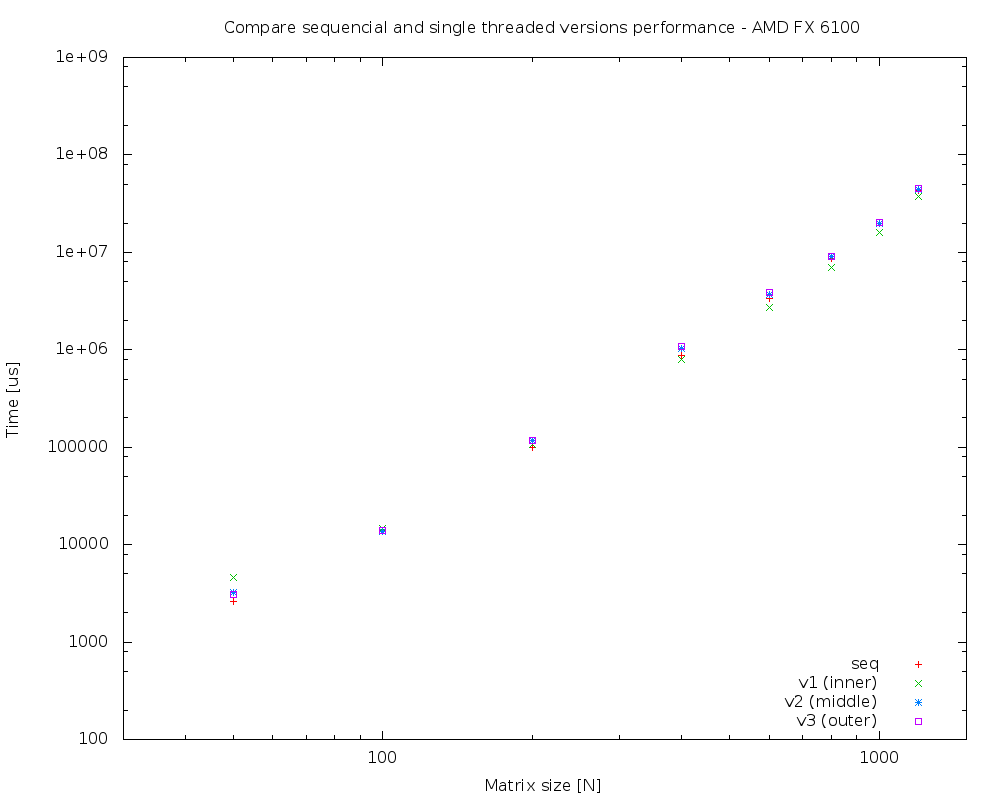
\includegraphics[width=\textwidth]{cmp_single_thread_HAL}
        \caption{A gull}
        \label{fig:gull}
    \end{subfigure}%
    ~ %add desired spacing between images, e. g. ~, \quad, \qquad, \hfill etc.
    %(or a blank line to force the subfigure onto a new line)
    \begin{subfigure}[b]{0.3\textwidth}
        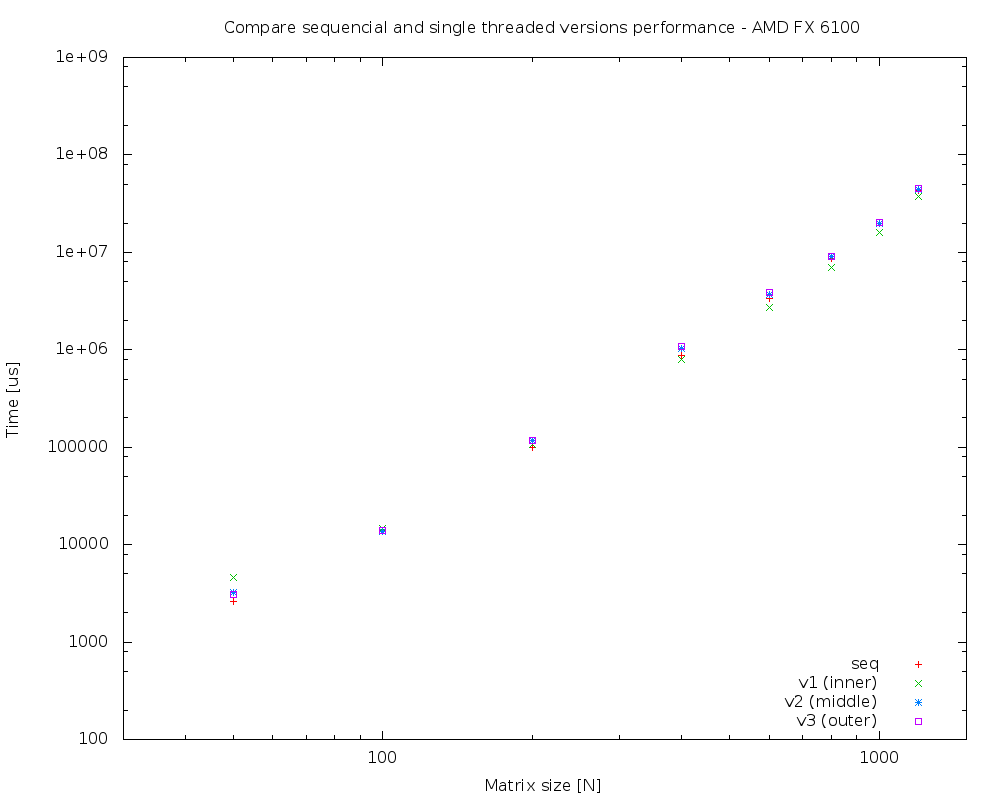
\includegraphics[width=\textwidth]{cmp_single_thread_HAL}
        \caption{A tiger}
        \label{fig:tiger}
    \end{subfigure}
    ~ %add desired spacing between images, e. g. ~, \quad, \qquad, \hfill etc.
    %(or a blank line to force the subfigure onto a new line)
    \begin{subfigure}[b]{0.3\textwidth}
        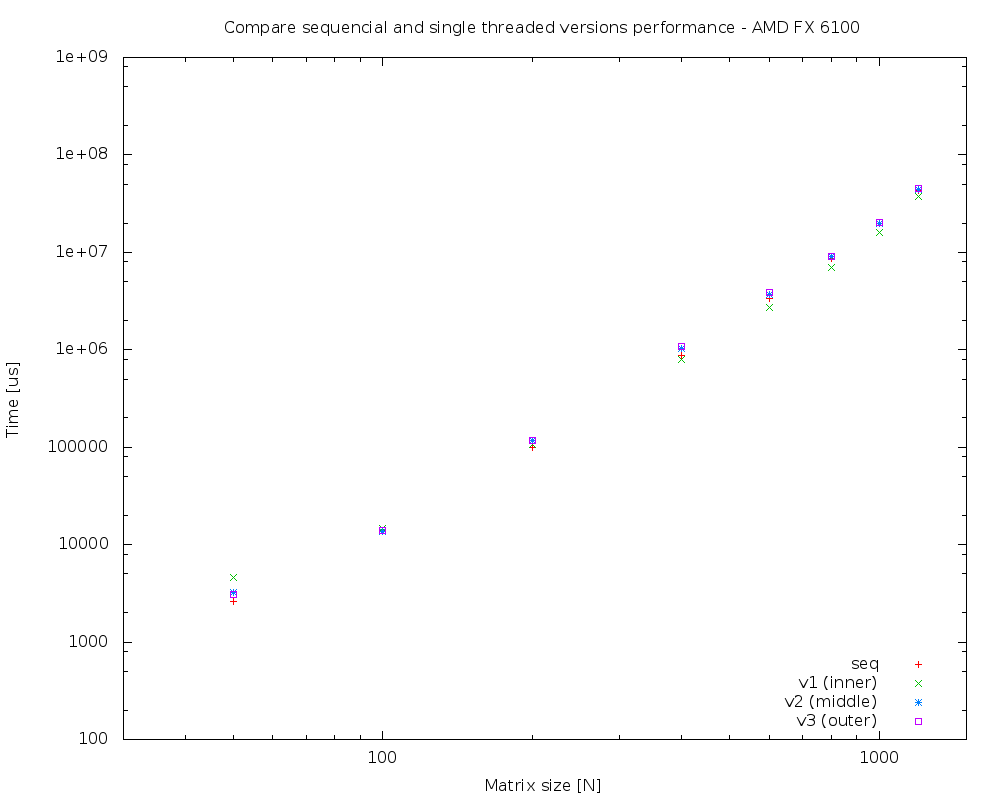
\includegraphics[width=\textwidth]{cmp_single_thread_HAL}
        \caption{A mouse}
        \label{fig:mouse}
    \end{subfigure}
    \caption{Pictures of animals}\label{fig:animals}
\end{figure}

\subsubsection{Paralelização do Laço mais Interno}

\subsubsection{Paralelização do Laço do Meio}

\subsubsection{Paralelização do Laço mais Externo}

\subsection{Conclusões} \label{sec:dis}

%\newpage
%\bibliographystyle{plainnat}
%\bibliography{relatorio}

\end{document}
